\chapter{Complex Numbers}

\begin{definitionbox}
	\begin{Definition}[Complex Numbers]\label{Complex Numbers}
		We define complex numbers to the ordered pair of real numbers and where addition and multiplication are defined to be as follows:

		\[
			\begin{split}
			\left( a,b \right) + \left( c,d  \right) &= \left( a+c, b+d \right) \\
			\left( a,b \right)  \left( c,d  \right) &= \left( ad-bc, ac+bd \right) 
			\end{split}
		.\]

		It is easily checked that this is in fact a field.
		where the multiplicative identity is $\left( 1,0 \right)$ and the additive identity is $\left( 0, 0 \right) $. 
	\end{Definition}
\end{definitionbox}

If we put $\left( a,b \right) $ as $a+ib$ where $i = (0,1)$ then we can totally abandon the ordered pair notation and perform simple algebra keeping in mind that $i^2 = -1$. \\

Often in copmlex analysis we will be concerned with functions that become $\infty$ when the function approaches a certain given point. To make this notion of distance more formal, we introduce the extended plane  which is the $\C \cup \left\{\infty \right\}  = \C_\infty$

\begin{center}
	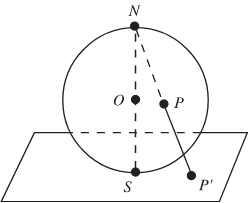
\includegraphics{img/Unknown.png}
\end{center}

Let $N = \left( 0,0,1 \right) $ that is, $N$ is the north pole on $S$. We can identify $\C$ with $\left( x_1, x_2 \right); x_1, x_2 \in  \mathbb{R}$ so that $\C$ cuts $S$ along the equatorial  plane. Now for each point $z \in \C$ consider the straight line in $\mathbb{R}^3$ through $z$ and $N$. This intersects the sphere exactly at one point. $Z \neq N$. If $ \abs{z} > 1$, the point on the sphere must lie in the northern hemisphere and if the point lies in the southern hemisphere, it must lie in the southern hemisphere. It is apparent that as $\abs{z} \to \infty$, $Z$  approaches $N$. Hence, we identify $N$ as the point $\infty$ in $\C_\infty$. \\


Given a point $z$ in $\C$  we can identify the corresponding point $Z$ in $S$ as follows:


\[
	x_1 = \frac{z + \overline{z}}{\abs{z}^2 +1}, x_2= \frac{-i(z - \overline{z})}{\abs{z}^2 +1}, x_3 =  \frac{\abs{z}^2 -1}{\abs{z}^2 +1}
.\] 

Similarly, if we have a point $Z$ in $S / \left\{ \infty \right\} $, the corresponding point in $\C$ as 

\[
z = \frac{x_1 + i x_2}{1-x_3}
.\]
Now we slightly modify the definition of distance in $\C_\infty$ as follows: For $z_1, z_2  \in  \C_\infty$, we have $d(z_1,z_2) = $ the distance between the corresponding points in $\mathbb{R}^3$
Now it is easy to show that distance between two point $z_1, z_2 \in \C$ is equal to the following in $S$:

\[
	\frac{2 \abs{z_1 - z_2}}{\sqrt{1 + z_1^2} \sqrt{1 + z_2^2}} 
.\]

And in a similar way, we get that :

\[
	d\left( z, \infty \right)  =  \frac{2}{\sqrt{1+\abs{z}^2} }
.\]

This correspondence between $S$ and $\C_\infty$ as the stereographic projection.

